\documentclass[fleqn,reqno,10pt]{article}

\usepackage{myarticlestyledefault}

\usetikzlibrary{calc}

\title{A Bayesian model for the K2 data}
\author{}
\date{}

\begin{document}
\maketitle

\section{The new data}

We have 40 participants with 86 data points each. We should exclude 2
participants (VPs 2 and 29) due to bad overal performance (more than
40\% errors on controls and target-related fillers). The mean success
rate on positional controls after this exclusion is $.91$. The
observed answer patterns are:

\medskip

\begin{minipage}[t]{0.45\linewidth}
\begin{verbatim}
     lit loc glb false
as-n 100   6   0     8
as-a  95  11   2     6
es-n  65  13   0    36
es-a  73  21   0    20
\end{verbatim}
\end{minipage}
\begin{minipage}[t]{0.45\linewidth}
\begin{verbatim}
   late early false
ee   60    39    33
el  114    12     8
en   93    20    19
le   52    61    19
ll  108    14    12
ln   84    32    16
\end{verbatim}
\end{minipage}

\medskip

There are no longer glaring individual consistencies in answer
patterns. The contingency table for AS-N and ES-N conditions that we
had in the paper before, now looks as follows:
\begin{verbatim}
                           ES-N
AS-N           inconsistent literalist localist
  inconsistent            0          1        2
  literalist              5         26        3
  localist                0          0        1
\end{verbatim}
The same information for AS-A vs.~ES-A:
\begin{verbatim}
                           ES-A
AS-A           inconsistent literalist localist
  inconsistent            1          0        5
  literalist              2         28        1
  localist                0          0        1
\end{verbatim}
Across all critical conditions we only have one consistent localist
(VP 22):
\begin{verbatim}
inconsistent   literalist     localist 
          12           25            1 
\end{verbatim}

\section{A Bayesian model}

\paragraph{Motivation.} Our previous analysis did not really take into
account that choices are made in sequence. We hypothesized that there
might be a bias that VPs exit as early as possible, but we could not
operationalize or even \textbf{quantify} that bias. Of course, this is why we
had the target-related fillers. This way we could at least make sure
whether everybody would exit at the earliest possible position.

Our main argument is about three conceivable readings and how
accessible / salient / strong they are in relation to each other. We
wanted to conclude that our old data suggests that we get an ordering
like so: LIT > LOC > (GLB), where we left it open as to whether GLB
was attested (Sec.~5.6, p.~32, in (23)). This was the main leverage
for saying that neither traditionalism, nor grammaticalism predict are
entirely correct: they both fail to predict that preference
relation. Unfortunately, the conclusion that our data suggests this
preference relation was rather indirect. In any case, there was no
chance to \textbf{quantify} exactly how much more salient LIT was than
LOC, for example.

\paragraph{The model.} Here is a very simple probabilistic model that
quantifies the positional bias and the competing strength of available
readings. Take the AS-conditions as an example. There are three
potential readings. Let's assume that the relative strength between
these is given by a probability vector $\myvec{p}^\text{as-n} =
\tuple{p^\text{as-n}_{\text{lit}},p^\text{as-n}_{\text{loc}},p^\text{as-n}_{\text{glb}}}$. We
assume that when a subject is at a critical position where, say, the
literal reading can be judged true or false, then the subject's
probability of giving the right judgment at that position is
proportional to $p^\text{as-n}_{\text{lit}}$. In other words, if there
were no potential effects of sequentiality and no errors, the vector
$\myvec{p}^\text{as-n}$ would be our prediction of observed
frequencies of in answer patterns. We look at four such three-placed
vectors, one for each target condition.

For each preference-related control condition $k$, we look at a
two-placed vector of the form $p^k =
\tuple{p^{\text{k}}_{\text{late}},
  p^{\text{k}}_{\text{early}}}$. However, since conditions $EX$ and
$LX$ (with $X \in \set{E,L,N}$) differ only with respect to the order
in which readings can be judged, the underlying relative strengths of
readings, and hence the relevant vectors, are taken to be identical.

To add potential effects of sequentiality, we assume that there is a
factor $q \in [0;1]$ that is constant over all conditions with which a
reading that can be judged first is amplified (if $q > .5$) or
de-amplified (if $q <.5$). We may hypothesize that subjects like to
exit as early as possible ($q$ is almost one), but we don't know for
sure, so we let the data decide what we should believe eventually. In
the AS-sequences, LIT can be judged first, then LOC and then GLB. So
we will assume that $p_{\text{lit}}$ is multiplied by $q$, that
$p_{\text{loc}}$ is multiplied by $(1-q)q$ and that $p_{\text{glb}}$
is multiplied by $(1-q)^2$.

Finally, we also allow for the chance of subjects making mistakes. We
should first keep things as simple as possible (no consideration for
spill-overs, late decisions, preferences to unravel completely before
judging etc.). So we assume that there is a fixed error rate $e^k \in
[0;1]$ for each condition $k$ with which subjects make wrong decisions
along the sequence. We allow for different error rates for different
conditions, because it is known, for example, that non-monotonic
quantifiers are harder to process. A decision can be wrong but
incidentally coincide with a reading that is indicative of a relevant
reading. Error rates multiply in proportion to the number of steps in
a sequence: more choice, more chance to be wrong.

Taking this together we calculate, for each critical condition $k$ a
target probability vector $\myvec{t}^k =
\tuple{t^k_{\text{lit}},t^k_{\text{loc}},t^k_{\text{glb}},t^k_{\text{err}}}$
with which we expect an answer to be classified as LIT, LOC, GLB or as
an error. For example, for AS-N, where LIT can be judged before GLB
before LOC, we get:
\begin{align*}
  t^{\text{as-n}}_{\text{lit}} & \propto q \
  p^\text{as-n}_{\text{lit}} + e^\text{as-n} &   t^{\text{as-n}}_{\text{loc}} & \propto (1-q)^2 \
  p^\text{as-n}_{\text{loc}} + e^\text{as-n} \\
  t^{\text{as-n}}_{\text{glb}} & \propto (1-q) \
  p^\text{as-n}_{\text{glb}} + e^\text{as-n} &   t^{\text{as-n}}_{\text{err}} &
  \propto 12 e^\text{as-n}
\end{align*}
Two remarks. The vector $\myvec{t}^k$ should be normalized eventually,
which is why $\propto$ is used instead of $=$. Also, the probability
of error $t^{\text{as-n}}_{\text{err}}$ comes from the observation
that there are 15 positions in total in an AS-sequence at which
subjects can make an erroneous choice, but we have accounted for three
of these already as adding to the count of answers indicative of
relevant readings.

Similarly, we compute a target probability $\myvec{t}^k =
\tuple{t^k_{\text{late}},t^k_{\text{early}},t^k_{\text{err}}}$ for
each preference-related control condition $k$, taking into account
which reading can be judged first and the length of the respective
sequences.

The full probabilistic model is visualized in
Figure~\ref{fig:model_graph}. As indicated there, we assume largely
uninformative priors. Any positional bias $q \in [0;1]$ is assumed to
be equally likely. The error rates for each condition should be small,
so we sample uniformly from interval $[0,.2]$. The biases
$\myvec{p}_k$ are also determined uniformly at random, by sampling from a
Dirichlet distribution with equal weights on all dimensions.

\begin{figure}[t]
  \centering
  \begin{tikzpicture}[node distance = 2.5cm, 
    double distance = 2pt,
    minimum size=1.25cm,
    thick]
    
    \node[rectangle, draw=black, fill=black!30] (obs)
    {obs$_k$};

    \node[rectangle, draw=black, fill=black!30,
    right of = obs] (n) {$n_k$};

    \node[below of = n, node distance= 1.5cm]
    (anchor) {};

    \node[left of = anchor, node distance= 0.5cm] (k) {$k \in
      \set{\text{as-n, as-e, \dots}}$};

    \node[circle, double, draw=black,
    above of = obs] (t) {$\myvec{t}_k$};

    \node[circle, draw=black, 
    above of = t] (p) {$\myvec{p}_k$};

    \node[circle, draw=black, 
    right of = p] (e) {$e_k$};

    \node[circle, draw=black, 
    left of = p] (q) {$q$};

    \draw[->] (t)--(obs);

    \draw[->] (n)--(obs);

    \draw[->] (q)--(t);

    \draw[->] (p)--(t);

    \draw[->] (e)--(t);

    \begin{pgfonlayer}{background}
       \node [rounded corners,
       very thick,draw=black!40,fit={($(obs.south)+(0,-30pt)$) 
                                 ($(n.east)+(+5pt,0)$) 
                                 ($(e.north)+(0,+5pt)$) 
                                 ($(p.west)+(-5pt,0)$)}] {};
    \end{pgfonlayer}

    \begin{scope}[xshift = 7.5cm, node distance = 1cm]

      \node[] (obsd) {$\text{obs}_k \sim \text{Multinomial}(\myvec{t}_k,n_k)$};

      \node[above of = obsd] (td) {$\myvec{t}_k = \text{as described
          in text}$};

      \node[above of = td] (pd) {$\myvec{p}_k =
        \text{Dirichlet}(\tuple{\nicefrac{1}{k}, \nicefrac{1}{k}, \dots})$};

      \node[above of = pd] (ed) {$e_k \sim \mathcal{U}(0,.2)$};

      \node[above of = ed] (qd) {$q \sim \mathcal{U}(0,1)$};



    \end{scope}

  \end{tikzpicture}
  \caption{Probabilistic graphical model}
  \label{fig:model_graph}
\end{figure}

\section{Analysis}

\begin{figure}
  \centering
  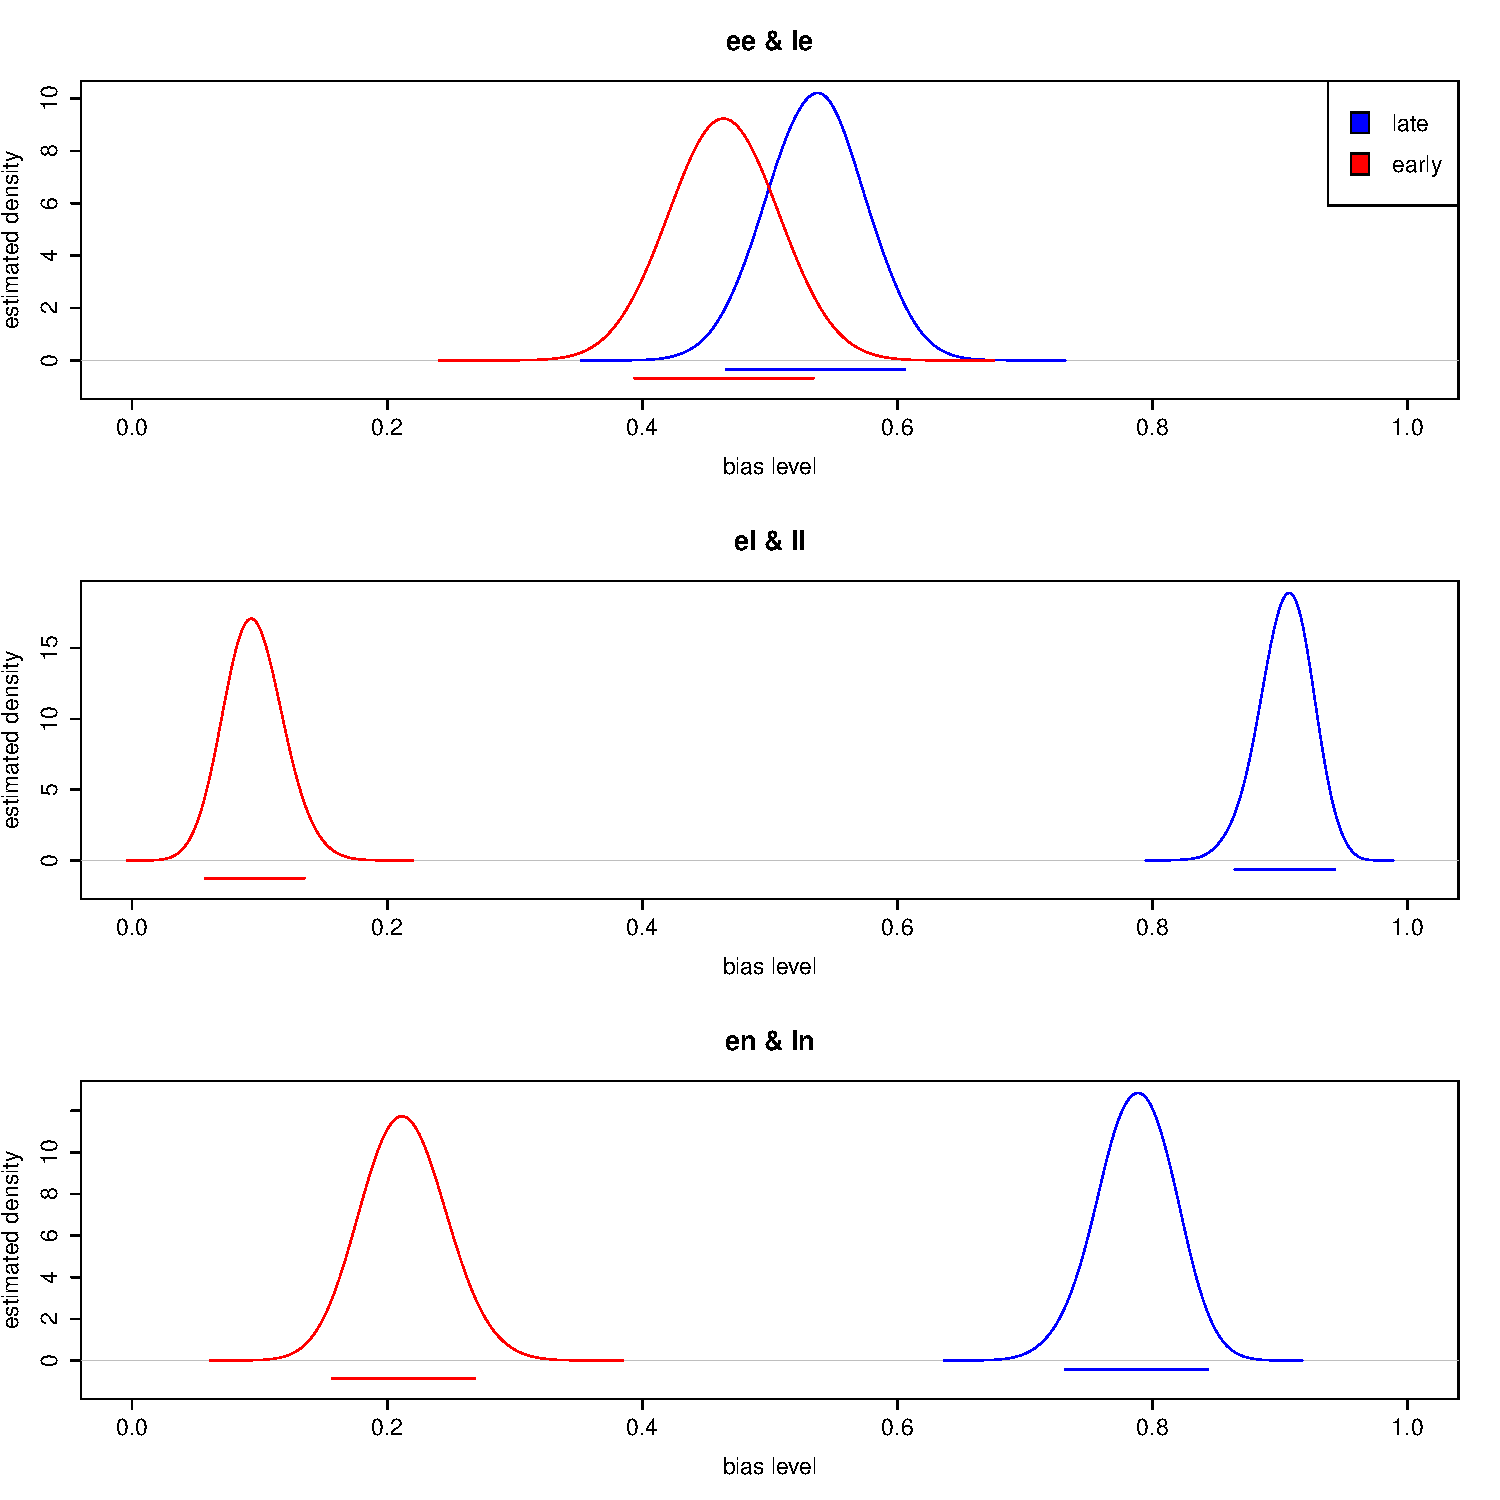
\includegraphics[width=\textwidth]{pics/Posterior_TF.pdf}
  \caption{Posterior over weights for target readings in
    target-related control conditions.}
  \label{fig:Posterior_TF}
\end{figure}

Using MCMC sampling, we obtain estimates for the posterior of the
latent parameters given the data. We are most interested in the level
of credence we should place on the weights of target readings in
critical conditions. But to check whether the model yields sensible
results we first look at the preference-related control
conditions. 

Estimates for the posteriors over weights for target-related controls
are plotted in Figure~\ref{fig:Posterior_TF}. The results are exactly
as we would expect them to be. Given our data, we should believe that
the late-closure reading is more prominent. But the level of
prominence varies with accentuation. Under prosody that we
hypothesized would favor the late-closure reading, the contrast is
most pronounced. Contrarily, accentuation that we hypothesized favors
the early-closure reading we are no longer justified in believing that
the late-closure reading is certainly preferred (witness the clearly
overlapping 95\% confidence regions).

\begin{figure}
  \centering
  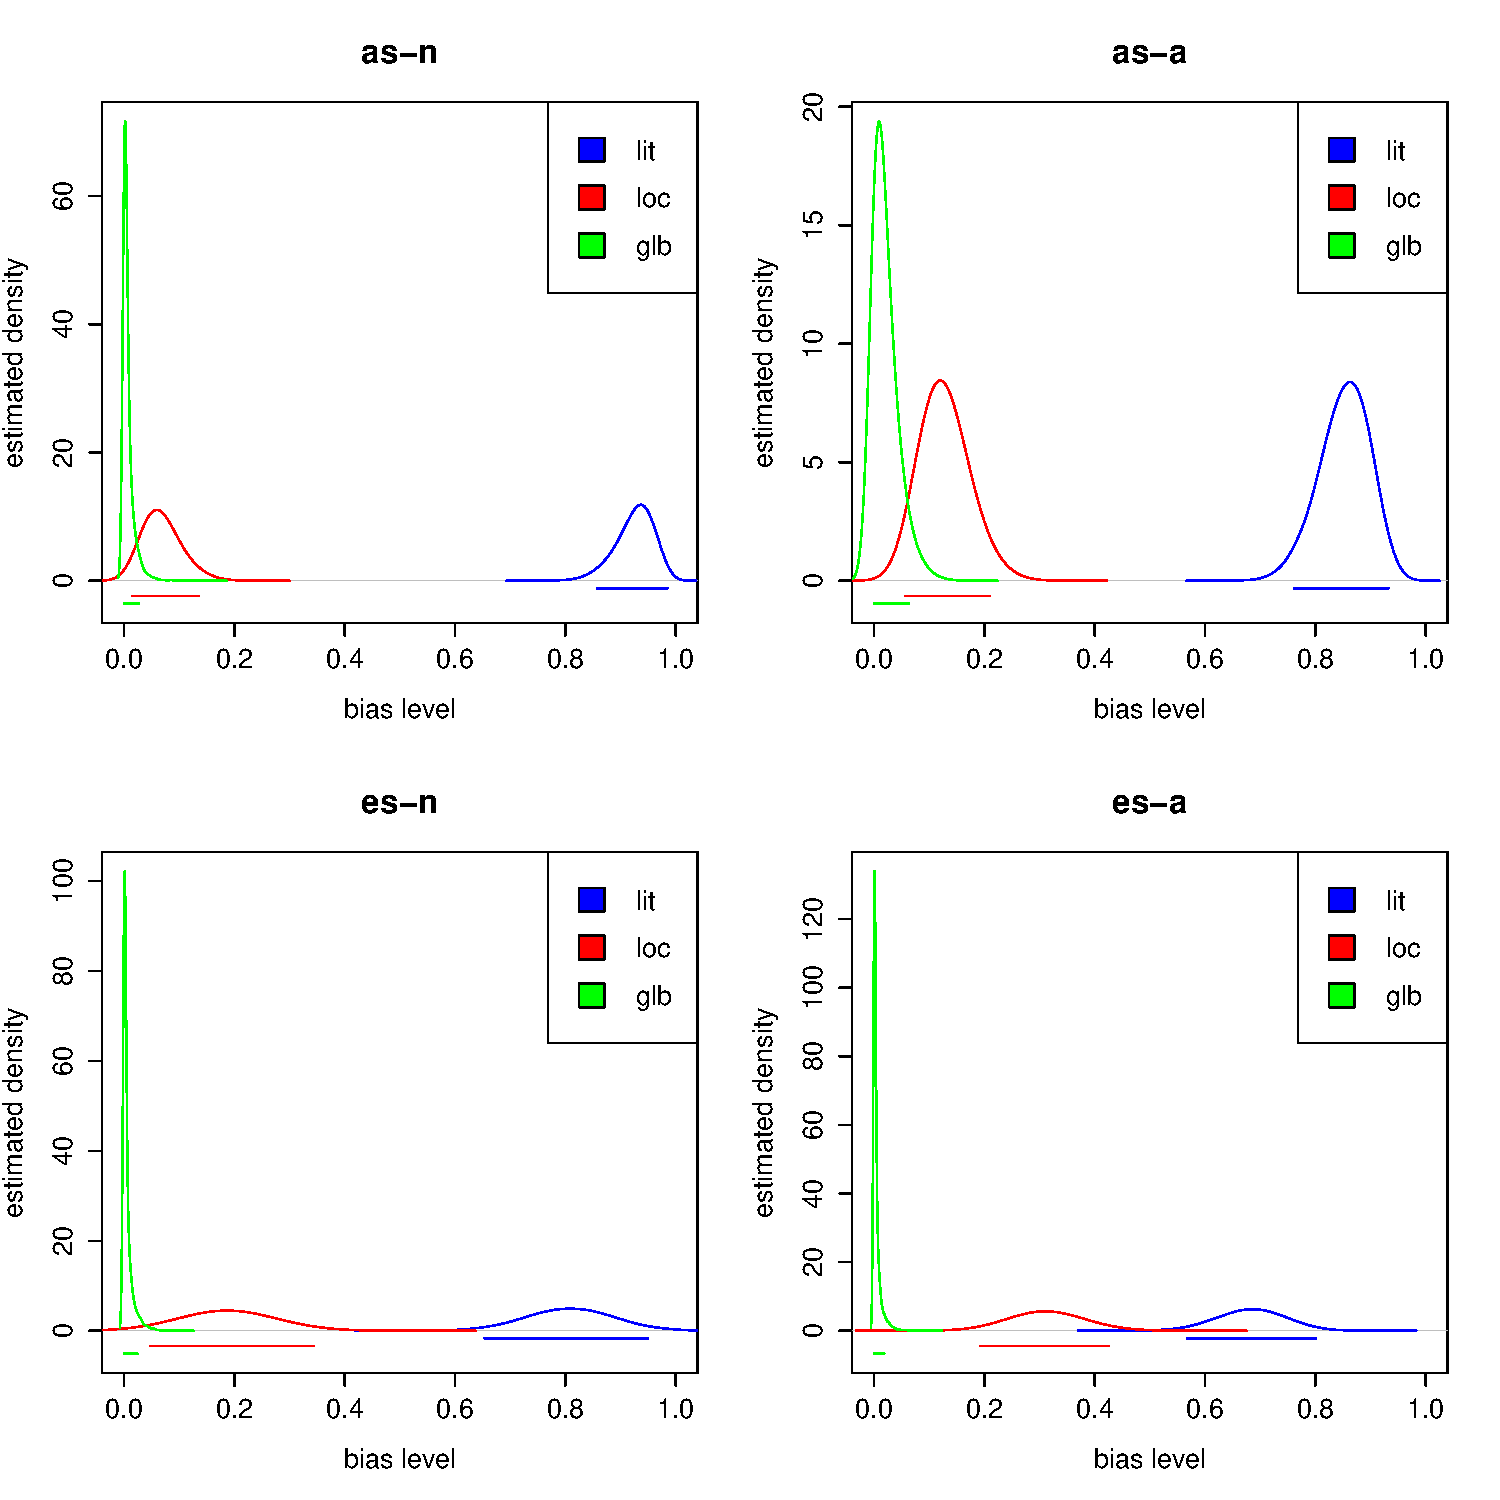
\includegraphics[width=\textwidth]{pics/Posterior_T.pdf}
  \caption{Posteriors over weights for target readings in critical
    conditions. Colored lines below the actual plots indicate 95\%
    confidence intervals.}
  \label{fig:Posterior_T}
\end{figure}

Turning to the critical conditions, estimates of posteriors over
weights given our data are given in Figure~\ref{fig:Posterior_T}. We
only have marginal reasons to believe that global readings have any
non-negligible weight data in the AS-A condition. Apart from this, if
the model is true, the data corroborates the belief that the literal
reading is strongly preferred over the local reading over the global
reading (again witness the non-overlapping 95\% confidence
regions). We also see the expected general effect of intonational
markedness. Qualitatively speaking, the preference for literal
readings appears less pronounced in the accented conditions.

\todo[inline]{still to be added: posteriors over $q$ and errors $e_k$}

\paragraph{Model validation.} We should also check whether the model
is actually a suitable model to predict the observed data. Posterior
predictive checks indicate that it is. Figures~\ref{fig:Posterior_TF}
and \ref{fig:Posterior_T} show simulated samples of answer patterns
that the model predicts under the posterior values for the latent
parameters. Everything looks almost perfect, with the only exception
the estimation of global readings in the ES-conditions.

\begin{figure}
  \centering
  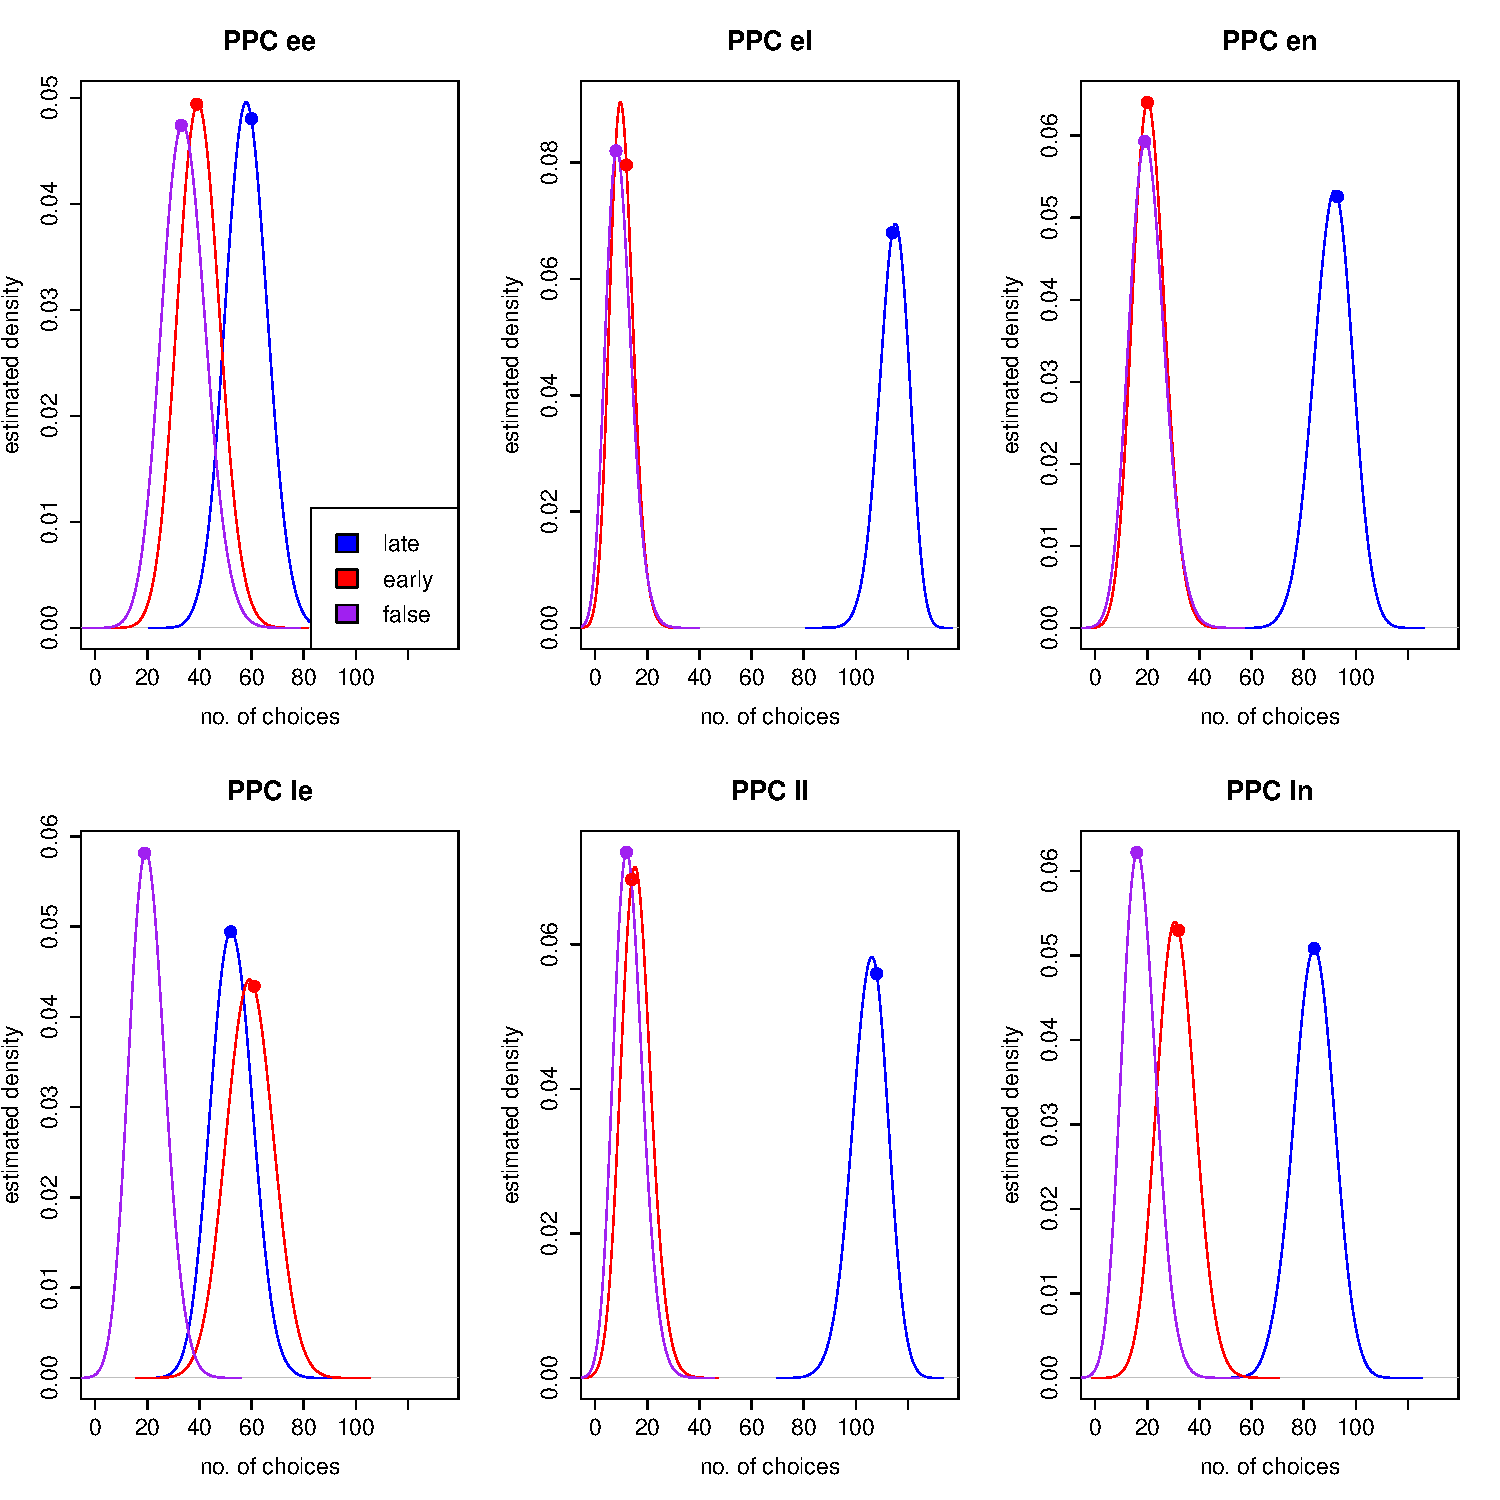
\includegraphics[width=\textwidth]{pics/PPC_TF.pdf}
  \caption{Posterior predictive check for the target-related control
    conditions. The colored dots on the plots indicate the actual
    observed numbers of choices. Intuitively speaking, the ``higher''
    the dot on the curve, the more likely does the model (under the
    posterior values for its parameters) predict the data (on which
    the posterior estimate is based).}
  \label{fig:Posterior_TF}
\end{figure}


\begin{figure}
  \centering
  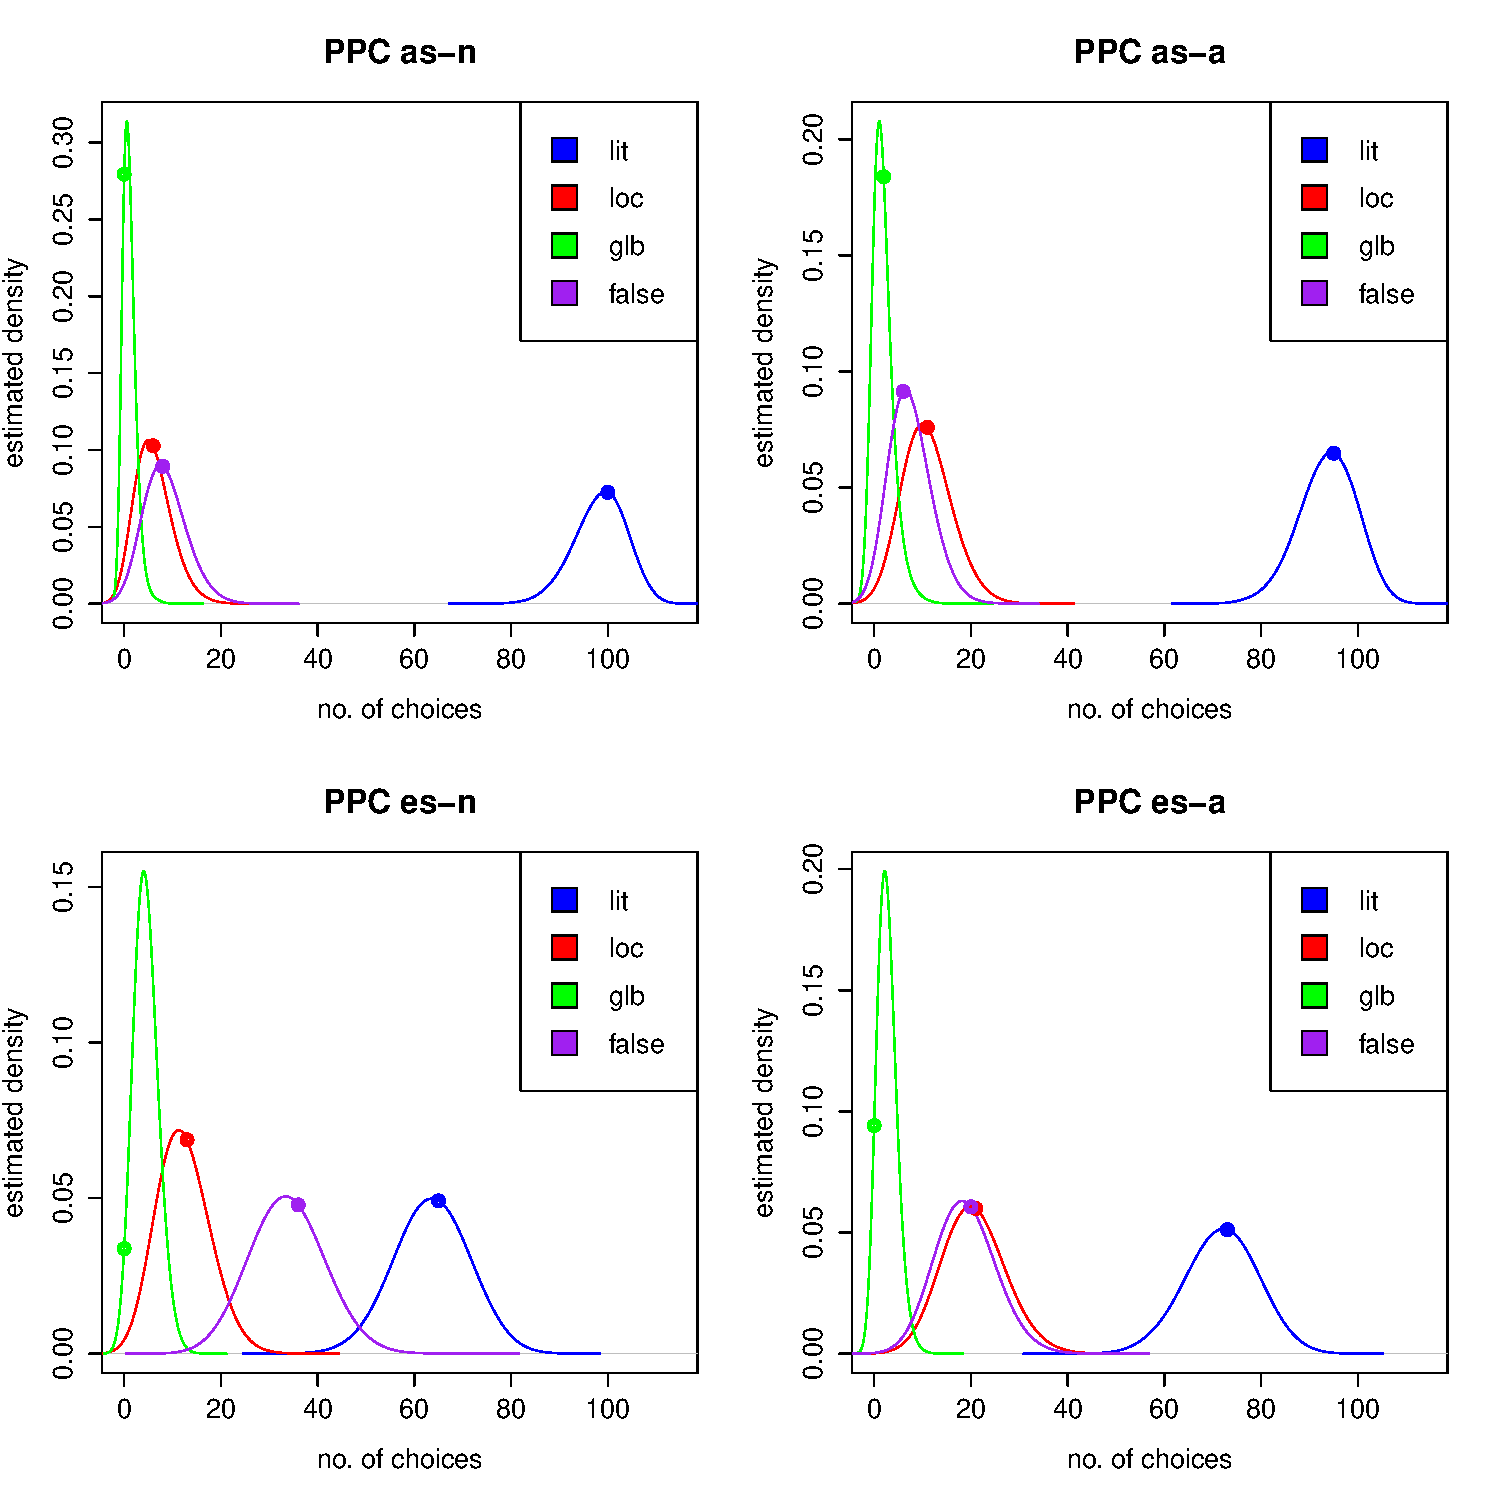
\includegraphics[width=\textwidth]{pics/PPC_T.pdf}
  \caption{Posterior predictive check for the target-related control
    conditions.}
  \label{fig:Posterior_T}
\end{figure}

\printbibliography[heading=bibintoc]

\end{document}
